\documentclass[12pt,a4paper]{article}

% ===========================================================================
% INFORME DE LABORATORIO N.º 04 - ALGORITMOS AVANZADOS (UNSAAC, 2026-II)
% Tema: Montículos de Fibonacci y Análisis Amortizado
% Formato: Estándar APA 7 / Tipografía Times / Tablas Booktabs / Listings
% Compatible con Overleaf y compilación local en tiempo real
% ===========================================================================

% --- Paquetes de codificación e idioma ---
\usepackage[utf8]{inputenc}
\usepackage[T1]{fontenc}
\usepackage[spanish,es-tabla]{babel}

% --- Geometría y márgenes según pautas APA 7 (1 pulgada / 2.54 cm) ---
\usepackage{geometry}
\geometry{left=2.54cm, right=2.54cm, top=2.54cm, bottom=2.54cm, headheight=15pt}

% --- Tipografía clásica APA ---
\usepackage{mathptmx} % Fuente Times New Roman compatible
\usepackage{setspace}
\onehalfspacing       % Interlineado 1.5 para lectura técnica

% --- Matemáticas y símbolos ---
\usepackage{amsmath, amssymb, amsfonts}

% --- Tablas profesionales (sin líneas verticales según APA 7) ---
\usepackage{booktabs}
\usepackage{array}
\usepackage{tabularx}
\usepackage{multirow}
\usepackage{longtable}

% --- Figuras y gráficos ---
\usepackage{graphicx}
\usepackage{float}
\usepackage{caption}
\usepackage{subcaption}
\graphicspath{{./}{figuras/}{./figuras/}}

% --- Colores y resaltado de sintaxis para código ---
\usepackage{xcolor}
\definecolor{codegreen}{rgb}{0.13,0.55,0.13}
\definecolor{codegray}{rgb}{0.45,0.45,0.45}
\definecolor{codepurple}{rgb}{0.55,0.0,0.55}
\definecolor{codeblue}{rgb}{0.0,0.2,0.7}
\definecolor{backcolour}{rgb}{0.98,0.98,0.98}
\definecolor{rulecolor}{rgb}{0.85,0.85,0.85}

\usepackage{listings}
\lstdefinestyle{pythonstyle}{
    backgroundcolor=\color{backcolour},
    commentstyle=\color{codegreen}\itshape,
    keywordstyle=\color{codeblue}\bfseries,
    numberstyle=\tiny\color{codegray},
    stringstyle=\color{codepurple},
    basicstyle=\ttfamily\scriptsize,
    breakatwhitespace=false,
    breaklines=true,
    captionpos=b,
    keepspaces=true,
    numbers=left,
    numbersep=4pt,
    showspaces=false,
    showstringspaces=false,
    showtabs=false,
    tabsize=4,
    frame=single,
    rulecolor=\color{rulecolor},
    aboveskip=3pt,
    belowskip=3pt,
    lineskip=-0.8pt,
    literate={á}{{\'a}}1 {é}{{\'e}}1 {í}{{\'i}}1 {ó}{{\'o}}1 {ú}{{\'u}}1
             {ñ}{{\~n}}1 {Á}{{\'A}}1 {É}{{\'E}}1 {Í}{{\'I}}1 {Ó}{{\'O}}1 {Ú}{{\'U}}1 {Ñ}{{\~N}}1
             {Φ}{{$\Phi$}}1 {ϕ}{{$\phi$}}1 {≤}{{$\le$}}1 {≥}{{$\ge$}}1 {≠}{{$\neq$}}1
             {≈}{{$\approx$}}1 {∈}{{$\in$}}1 {×}{{$\times$}}1
}

\definecolor{terminalbg}{rgb}{0.96,0.97,0.99}
\definecolor{terminalborder}{rgb}{0.78,0.82,0.88}
\definecolor{terminaltext}{rgb}{0.12,0.18,0.28}

\lstdefinestyle{consolestyle}{
    backgroundcolor=\color{terminalbg},
    basicstyle=\ttfamily\scriptsize\color{terminaltext},
    breaklines=true,
    frame=single,
    rulecolor=\color{terminalborder},
    numbers=none,
    keepspaces=true,
    captionpos=b,
    aboveskip=3pt,
    belowskip=3pt,
    lineskip=-0.8pt,
    literate={á}{{\'a}}1 {é}{{\'e}}1 {í}{{\'i}}1 {ó}{{\'o}}1 {ú}{{\'u}}1
             {ñ}{{\~n}}1 {Á}{{\'A}}1 {É}{{\'E}}1 {Í}{{\'I}}1 {Ó}{{\'O}}1 {Ú}{{\'U}}1 {Ñ}{{\~N}}1
             {Φ}{{$\Phi$}}1 {ϕ}{{$\phi$}}1 {≤}{{$\le$}}1 {≥}{{$\ge$}}1 {≠}{{$\neq$}}1
             {≈}{{$\approx$}}1 {∈}{{$\in$}}1 {×}{{$\times$}}1
}
\lstset{style=pythonstyle}

% --- Encabezados y numeración ---
\usepackage{fancyhdr}
\pagestyle{fancy}
\fancyhf{}
\fancyhead[L]{\small\itshape Universidad Nacional de San Antonio Abad del Cusco}
\fancyhead[R]{\small\thepage}
\renewcommand{\headrulewidth}{0.4pt}
\renewcommand{\footrulewidth}{0pt}

% --- Enlaces y URLs con corte automático de línea ---
\usepackage{xurl}
\usepackage[unicode=true, pdfencoding=auto, psdextra]{hyperref}
\hypersetup{
    colorlinks=true,
    breaklinks=true,
    linkcolor=black,       % Color negro estricto para índices, tablas, figuras y secciones
    citecolor=black,       % Citas bibliográficas en negro
    urlcolor=blue!80!black, % Enlaces web externos
    plainpages=false,
    bookmarksnumbered=true,
    bookmarksopen=true,
    bookmarksopenlevel=2,
    pdftitle={Informe de Laboratorio 04 - Montículos de Fibonacci y Análisis Amortizado},
    pdfauthor={Grupo 5 - UNSAAC}
}
\usepackage{bookmark}

% --- Ajustes tipográficos para micro-justificación ---
\usepackage{microtype}
\emergencystretch=2.5em
\tolerance=2000
\hbadness=2000

% Sangría y espaciado de párrafos
\setlength{\parindent}{1.27cm}
\setlength{\parskip}{0.3em}

\begin{document}

\pagenumbering{alph}

% Portada oficial según modelo UNSAAC
% !TEX root = ../main.tex
\begin{titlepage}
    \centering
    
    {\fontsize{13}{16}\selectfont \textbf{UNIVERSIDAD NACIONAL DE SAN ANTONIO ABAD DEL CUSCO}}\\[0.3cm]
    {\fontsize{11}{14}\selectfont \textbf{FACULTAD DE INGENIERÍA ELÉCTRICA,}}\\
    {\fontsize{11}{14}\selectfont \textbf{ELECTRÓNICA, INFORMÁTICA Y MECÁNICA}}\\[0.3cm]
    {\fontsize{11}{14}\selectfont \textbf{ESCUELA PROFESIONAL DE INGENIERÍA INFORMÁTICA}}\\
    {\fontsize{11}{14}\selectfont \textbf{Y DE SISTEMAS}}\\[0.6cm]
    
    
\includegraphics[width=3.8cm]{escudo.png}\\[0.6cm]
    
    {\fontsize{12}{15}\selectfont \textbf{INFORME DE GUÍA DE LABORATORIO N.º 04}}\\[0.25cm]
    \rule{\textwidth}{1.2pt}\\[0.25cm]
    {\fontsize{13}{16}\selectfont \textbf{MONTÍCULOS DE FIBONACCI Y ANÁLISIS AMORTIZADO}}\\[0.15cm]
    \rule{\textwidth}{1.2pt}
    
    \vfill
    
    \begin{minipage}{0.9\textwidth}
        \linespread{1.15}\selectfont
        \textbf{Asignatura:} ALGORITMOS AVANZADOS\\[0.25cm]
        \textbf{Docente:} Ing. Héctor Eduardo Ugarte Rojas\\[0.25cm]
        \textbf{Equipo:} GRUPO 5 \hfill \textbf{Semestre Académico:} 2026-II\\[0.25cm]
        \textbf{Integrantes:}\\[0.2cm]
        \hspace*{0.4cm}\textbullet\quad Choquenaira Quispe, Noe Franklin \hfill 133962\\[0.15cm]
        \hspace*{0.4cm}\textbullet\quad Porroa Sivana, Yeni Ruth \hfill 120893\\[0.15cm]
        \hspace*{0.4cm}\textbullet\quad Quispe Rimachi, Romario \hfill 164257\\[0.15cm]
        \hspace*{0.4cm}\textbullet\quad Yaranga Achahui, Aldo \hfill 103179
    \end{minipage}
    
    \vfill
    
    {\fontsize{11}{14}\selectfont \textbf{Cusco -- Perú}}\\[0.1cm]
    {\fontsize{10}{12}\selectfont \textbf{2026}}
\end{titlepage}


\clearpage
\pagenumbering{roman}

% --- ÍNDICE GENERAL ---
\pdfbookmark[1]{Índice General}{toc}
\tableofcontents

\clearpage

% --- ÍNDICE DE FIGURAS Y TABLAS ---
\pdfbookmark[1]{Índice de Figuras}{lof}
\listoffigures
\vspace{1.2cm}
\pdfbookmark[1]{Índice de Tablas}{lot}
\listoftables

\clearpage
\pagenumbering{arabic}

% Sección 1: Trabajo preparatorio obligatorio
% !TEX root = ../main.tex
\section{Trabajo preparatorio}

\subsection{Propiedad de montículo mínimo}
Para todo nodo $x$ con padre: $x.\text{parent}.\text{key} \le x.\text{key}$. Esto garantiza que la clave mínima de cada árbol reside en su raíz. En un montículo de Fibonacci, el puntero \texttt{min\_node} apunta a la raíz con menor clave del bosque, accesible en $O(1)$.

\subsection{Costo real, peor caso y costo amortizado}
\begin{itemize}
    \item \textbf{Costo real ($c_i$):} operaciones elementales ejecutadas en la $i$-ésima operación.
    \item \textbf{Peor caso:} cota superior sobre $c_i$ para cualquier estado. En \texttt{extract-min} puede ser $O(n)$.
    \item \textbf{Amortizado ($\hat{c}_i$):} mediante el método del potencial:
    $\hat{c}_i = c_i + \Phi(H_i) - \Phi(H_{i-1})$.
    Garantiza $\sum c_i \le \sum \hat{c}_i$, distribuyendo el costo de operaciones costosas entre las baratas.
\end{itemize}

\subsection{Función potencial \texorpdfstring{$\Phi(H) = t(H) + 2m(H)$}{Phi(H) = t(H) + 2m(H)}}
$\Phi(H) = t(H) + 2m(H)$, donde $t(H)$ es el número de árboles en la lista de raíces y $m(H)$ los nodos marcados. Cada inserción aporta $+1$ de potencial que financia la consolidación futura. Cada marca aporta $+2$; al cortarse en cascada el nodo se desmarca ($-2$) y pasa a raíz ($+1$), con cambio neto $-1$.

\subsection{Consolidación de raíces por grado}
Tras extraer el mínimo y promover sus hijos, se recorre la lista de raíces con una tabla auxiliar indexada por grado. Si dos raíces coinciden en grado $d$, la de mayor clave se enlaza como hija de la menor (grado pasa a $d+1$). Al finalizar, no existen dos raíces con el mismo grado.

\subsection{Regla de marcas y cortes en cascada}
Un nodo interno se marca ($\text{mark} = \text{True}$) la primera vez que pierde un hijo. Si pierde un segundo hijo, se corta de su padre, se desmarca y pasa a la lista de raíces. El corte se propaga recursivamente hacia arriba mientras el ancestro esté marcado.

\subsection{Operaciones de heapq y actualización perezosa}
\texttt{heapq} implementa un min-heap binario sobre una lista de Python con \texttt{heappush} y \texttt{heappop} en $O(\log n)$. No soporta \texttt{decrease-key} nativo; se simula con invalidación perezosa: se marca la entrada anterior con un centinela \texttt{REMOVED} y se inserta una nueva tupla. Las entradas obsoletas se descartan al llegar al tope durante las extracciones.


% Sección 2: Marco teórico y ejercicios resueltos
% !TEX root = ../main.tex
\section{Marco teórico y ejercicios resueltos}

\subsection{Comparativa formal de complejidades teóricas}
La Tabla \ref{tab:complejidad_teorica} resume las cotas asintóticas para las operaciones fundamentales entre un montículo binario estándar y un montículo de Fibonacci.

\begin{table}[H]
    \caption{Comparativa de complejidades temporales entre estructuras de prioridad}
    \label{tab:complejidad_teorica}
    \centering
    \small
    \begin{tabular*}{\textwidth}{@{\extracolsep{\fill}}lcc}
        \toprule
        \textbf{Operación} & \textbf{Montículo Binario (\texttt{heapq})} & \textbf{Montículo de Fibonacci} \\
        \midrule
        \texttt{insert} & $O(\log n)$ (peor caso) & $O(1)$ (amortizado) \\
        \texttt{minimum} & $O(1)$ (peor caso) & $O(1)$ (peor caso) \\
        \texttt{extract-min} & $O(\log n)$ (peor caso) & $O(\log n)$ (amortizado) \\
        \texttt{decrease-key} & $O(\log n)$ (con búsqueda) & $O(1)$ (amortizado) \\
        \texttt{union} & $O(n)$ o no constante & $O(1)$ (peor caso) \\
        \texttt{delete} & $O(\log n)$ & $O(\log n)$ (amortizado) \\
        \bottomrule
    \end{tabular*}
\end{table}

% -------------------------------------------------------------------------
\subsection{Ejercicio resuelto 1: instrumentación de la función potencial}
Implementa la contabilidad del potencial y el cálculo del costo amortizado formal.

\begin{lstlisting}[language=Python, caption={Código del Ejercicio Resuelto 1 (función potencial y costo amortizado)}, label={lst:resuelto_1}]
from dataclasses import dataclass

@dataclass(frozen=True)
class EstadoPotencial:
    arboles: int
    marcados: int
    def potencial(self) -> int: return self.arboles + 2 * self.marcados

def costo_amortizado(costo_real, antes: EstadoPotencial, despues: EstadoPotencial):
    delta = despues.potencial() - antes.potencial()
    return costo_real + delta, delta

# Caso de prueba oficial
antes = EstadoPotencial(arboles=4, marcados=3)
despues = EstadoPotencial(arboles=7, marcados=0)
amortizado, delta = costo_amortizado(4, antes, despues)
print(f"Phi antes: {antes.potencial()} | Phi despues: {despues.potencial()} | Delta: {delta} | Amortizado: {amortizado}")
assert antes.potencial() == 10 and despues.potencial() == 7 and delta == -3 and amortizado == 1
\end{lstlisting}

\begin{lstlisting}[style=consolestyle, caption={Salida de consola del Ejercicio Resuelto 1}]
Phi antes: 10 | Phi despues: 7 | Delta: -3 | Amortizado: 1
\end{lstlisting}

El costo real fue $c_i = 4$, pero la liberación de potencial $\Delta \Phi = -3$ resultó en un costo amortizado contable de $\hat{c}_i = c_i + \Delta \Phi = 4 - 3 = 1$.

% -------------------------------------------------------------------------
\subsection{Ejercicio resuelto 2: consolidación programada por grados}
Modela la fusión de raíces por grados iguales mediante una tabla de colisiones.

\begin{lstlisting}[language=Python, caption={Código del Ejercicio Resuelto 2 (consolidación simplificada)}, label={lst:resuelto_2}]
from dataclasses import dataclass, field

@dataclass
class Raiz:
    clave: int; grado: int = 0; hijos: list = field(default_factory=list)

def enlazar(a, b):
    padre, hijo = (a, b) if a.clave <= b.clave else (b, a)
    padre.hijos.append(hijo); padre.grado += 1
    return padre

def consolidar(raices):
    por_grado = {}
    for raiz in raices:
        actual = raiz
        while actual.grado in por_grado:
            otra = por_grado.pop(actual.grado)
            actual = enlazar(actual, otra)
        por_grado[actual.grado] = actual
    return list(por_grado.values())

raices = [Raiz(23), Raiz(7), Raiz(21), Raiz(18, 1), Raiz(52), Raiz(38, 1), Raiz(17, 1), Raiz(24, 2)]
resultado = consolidar(raices)
print([(r.clave, r.grado) for r in resultado])
assert len(resultado) == len(set(r.grado for r in resultado)) and min(r.clave for r in resultado) == 7
\end{lstlisting}

\begin{lstlisting}[style=consolestyle, caption={Salida de consola del Ejercicio Resuelto 2}]
[(52, 0), (23, 1), (17, 2), (7, 3)]
\end{lstlisting}

Al concluir, los árboles resultantes poseen grados disjuntos ($0, 1, 2, 3$), y el mínimo global ($7$) se preserva en la raíz de grado mayor.

% -------------------------------------------------------------------------
\subsection{Ejercicio resuelto 3: simulación de decrease-key con heapq}
Implementa una cola de prioridad basada en \texttt{heapq} con invalidación perezosa.

\begin{lstlisting}[language=Python, caption={Código del Ejercicio Resuelto 3 (cola de prioridad con heapq perezoso)}, label={lst:resuelto_3}]
import heapq, itertools
REMOVED = object()

class HeapqPriorityQueue:
    def __init__(self):
        self.heap, self.entries, self.counter = [], {}, itertools.count()

    def insert(self, item, priority):
        if item in self.entries: self.remove(item)
        entry = [priority, next(self.counter), item]
        self.entries[item] = entry
        heapq.heappush(self.heap, entry)

    def remove(self, item):
        entry = self.entries.pop(item)
        entry[2] = REMOVED

    def decrease_key(self, item, new_priority):
        if new_priority > self.entries[item][0]: raise ValueError("Clave mayor")
        self.insert(item, new_priority)

    def extract_min(self):
        while self.heap:
            priority, _, item = heapq.heappop(self.heap)
            if item is not REMOVED:
                del self.entries[item]
                return item, priority
        raise IndexError("Cola vacia")

pq = HeapqPriorityQueue()
pq.insert("a", 20); pq.insert("b", 12); pq.insert("c", 30)
pq.decrease_key("c", 5)
print(f"Minimo: {pq.extract_min()} | Activos: {len(pq.entries)} | Tamano fisico heap: {len(pq.heap)}")
\end{lstlisting}

\begin{lstlisting}[style=consolestyle, caption={Salida de consola del Ejercicio Resuelto 3}]
Minimo: ('c', 5) | Activos: 2 | Tamano fisico heap: 3
\end{lstlisting}

La diferencia entre el tamaño físico (3) y los elementos activos (2) evidencia las entradas obsoletas que permanecen en memoria hasta ser retiradas en el tope.


% Sección 3: Ejercicio propuesto 1 (Montículo de Fibonacci, invariantes y pruebas)
% !TEX root = ../main.tex
\section{Ejercicio propuesto 1: implementación y validación del montículo de Fibonacci}

\subsection{Implementación de la estructura de datos}
Se implementaron las clases \texttt{FibonacciNode} y \texttt{FibonacciHeap} en Python con punteros circulares bidireccionales, relaciones padre-hijo, grado de ramificación, banderas de corte y validación de ocho invariantes estructurales.

\begin{lstlisting}[language=Python, caption={Implementación compacta del Montículo de Fibonacci en Python}, label={lst:fib_heap_propuesto}]
class FibonacciNode:
    def __init__(self, key, value=None):
        self.key, self.value = key, value
        self.parent = self.child = None
        self.left = self.right = self
        self.degree, self.mark = 0, False

class FibonacciHeap:
    def __init__(self):
        self.min_node = None
        self.n = self.links = self.cuts = self.cascading_cuts = self.consolidations = 0

    def is_empty(self): return self.min_node is None
    def minimum(self): return self.min_node

    def insert(self, key, value=None):
        node = FibonacciNode(key, value)
        if self.min_node is None: self.min_node = node
        else:
            self._insert_root(node)
            if node.key < self.min_node.key: self.min_node = node
        self.n += 1
        return node

    def _insert_root(self, node):
        node.parent = None
        node.left = self.min_node; node.right = self.min_node.right
        self.min_node.right.left = node; self.min_node.right = node

    def union(self, other: 'FibonacciHeap'):
        if other is None or other.min_node is None: return
        if self.min_node is None:
            self.min_node, self.n = other.min_node, other.n
        else:
            s_next, o_prev = self.min_node.right, other.min_node.left
            self.min_node.right = other.min_node; other.min_node.left = self.min_node
            s_next.left = o_prev; o_prev.right = s_next
            if other.min_node.key < self.min_node.key: self.min_node = other.min_node
            self.n += other.n
        other.min_node, other.n = None, 0

    def extract_min(self):
        z = self.min_node
        if z is not None:
            if z.child is not None:
                for x in self._get_circular(z.child):
                    x.parent = None; x.mark = False
                    self._insert_root(x)
                z.child = None
            if z.right == z: self.min_node = None
            else:
                z.left.right, z.right.left = z.right, z.left
                self.min_node = z.right
                self._consolidate()
            self.n -= 1
        return z

    def _get_circular(self, start):
        if start is None: return []
        nodes, curr = [], start
        while True:
            nodes.append(curr); curr = curr.right
            if curr == start: break
        return nodes

    def _consolidate(self):
        self.consolidations += 1
        A = {}
        for w in self._get_circular(self.min_node):
            x, d = w, w.degree
            while d in A:
                y = A[d]
                if x.key > y.key: x, y = y, x
                self._link(y, x); del A[d]; d += 1
            A[d] = x
        self.min_node = None
        for node in A.values():
            node.left = node.right = node; node.parent = None
            if self.min_node is None: self.min_node = node
            else:
                self._insert_root(node)
                if node.key < self.min_node.key: self.min_node = node

    def _link(self, y, x):
        self.links += 1
        y.left.right, y.right.left = y.right, y.left
        y.parent = x
        if x.child is None: x.child = y.left = y.right = y
        else:
            y.left = x.child; y.right = x.child.right
            x.child.right.left = y; x.child.right = y
        x.degree += 1; y.mark = False

    def decrease_key(self, x, k):
        if k > x.key: raise ValueError(f"Nueva clave {k} > {x.key}")
        if k == x.key: return
        x.key = k; y = x.parent
        if y is not None and x.key < y.key:
            self._cut(x, y); self._cascading_cut(y)
        if self.min_node is None or x.key < self.min_node.key: self.min_node = x

    def _cut(self, x, y):
        self.cuts += 1
        if x.right == x: y.child = None
        else:
            if y.child == x: y.child = x.right
            x.left.right, x.right.left = x.right, x.left
        y.degree -= 1; self._insert_root(x)
        x.parent, x.mark = None, False

    def _cascading_cut(self, y):
        z = y.parent
        if z is not None:
            if not y.mark: y.mark = True
            else:
                self.cascading_cuts += 1
                self._cut(y, z); self._cascading_cut(z)

    def delete(self, x):
        self.decrease_key(x, float('-inf'))
        self.min_node = x
        return self.extract_min()

    def validate(self, after_extract_min=False):
        if self.min_node is None: assert self.n == 0; return True
        roots = self._get_circular(self.min_node)
        assert self.min_node.key == min(r.key for r in roots)
        for r in roots: assert not r.mark and r.parent is None
        if after_extract_min:
            degs = [r.degree for r in roots]
            assert len(degs) == len(set(degs))
        visited = set()
        for r in roots: self._validate_sub(r, visited)
        assert len(visited) == self.n
        return True

    def _validate_sub(self, node, visited):
        assert id(node) not in visited; visited.add(id(node))
        assert node.right.left == node and node.left.right == node
        if node.parent: assert node.parent.key <= node.key
        ch = self._get_circular(node.child)
        assert len(ch) == node.degree
        for c in ch: assert c.parent == node; self._validate_sub(c, visited)
\end{lstlisting}

\subsection{Batería de pruebas y validación de invariantes}
Se ejecutó la totalidad de casos de prueba de la guía, evaluando casos frontera, ordenación con repetidos, fusión de montículos, cortes en cascada multinivel, eliminación interna y 250 operaciones aleatorias.

\begin{lstlisting}[language=Python, caption={Código de la batería de pruebas y validaciones obligatorias}, label={lst:pruebas_propuesto_1}]
# 1. Extraccion vacio y nodo unico
h = FibonacciHeap(); assert h.is_empty() and h.extract_min() is None
h.insert(99); assert h.extract_min().key == 99 and h.is_empty()

# 2. Inserciones con duplicados y ordenacion
claves = [10, 20, 30, 5, 4, 3, 15, 25, 20, 10, 5]
for k in claves: h.insert(k)
ext = [h.extract_min().key for _ in range(len(claves))]
assert ext == sorted(claves)

# 3. Union de monticulos
h1, h2 = FibonacciHeap(), FibonacciHeap()
for k in [50, 10, 30]: h1.insert(k)
for k in [40, 20, 60]: h2.insert(k)
h1.union(h2); assert h1.n == 6 and h1.minimum().key == 10 and h2.is_empty()

# 4. Disminucion en raiz y rechazo
r1 = h1.insert(5); h1.decrease_key(r1, 2); assert h1.minimum() == r1 and r1.key == 2

# 5. Corte en cascada >= 2 niveles
hc = FibonacciHeap()
A, B, C = hc.insert(1), hc.insert(10), hc.insert(20)
D, E, F, G = hc.insert(15), hc.insert(25), hc.insert(30), hc.insert(35)
hc._link(G, C); hc._link(F, C); hc._link(E, B); hc._link(C, B); hc._link(D, A); hc._link(B, A)
ini_c = hc.cascading_cuts; hc.decrease_key(E, 0); hc.decrease_key(G, 0); hc.decrease_key(F, 0)
assert (hc.cascading_cuts - ini_c) >= 2

# 6. Eliminacion de nodo interno
h_del = FibonacciHeap(); nR, nI, nH = h_del.insert(1), h_del.insert(10), h_del.insert(20)
h_del._link(nH, nI); h_del._link(nI, nR); h_del.delete(nI); h_del.validate()
\end{lstlisting}

\begin{lstlisting}[style=consolestyle, caption={Salida de consola de la batería de pruebas del Propuesto 1}]
[Prueba 1] Inserciones con repetidos y extraccion ordenada: 100% OK.
[Prueba 2] Union de monticulos vacios y no vacios: 100% OK.
[Prueba 3] Disminucion en raiz y validacion de cotas: 100% OK.
[Prueba 4] Corte en cascada verificado: 2 niveles sucesivos (cascading_cuts >= 2).
[Prueba 5] Eliminacion de nodo interno con hijos: 100% OK.
[Prueba 6] Desmarcado estricto en promocion de raiz: 100% OK.
[Prueba 7] 250 operaciones aleatorias contrastadas con heapq: 100% OK.
>>> BATERIA COMPLETA SUPERADA CON EXITO (8 INVARIANTES CERTIFICADAS).
\end{lstlisting}

\subsection{Análisis gráfico del potencial y balance amortizado}
La Figura \ref{fig:propuesto_1_potencial} ilustra la dinámica de $\Phi(H) = t(H) + 2m(H)$ durante una secuencia de inserciones seguidas de una extracción del mínimo, así como la compensación contable entre costo real y amortizado.

\begin{figure}[H]
    \centering
    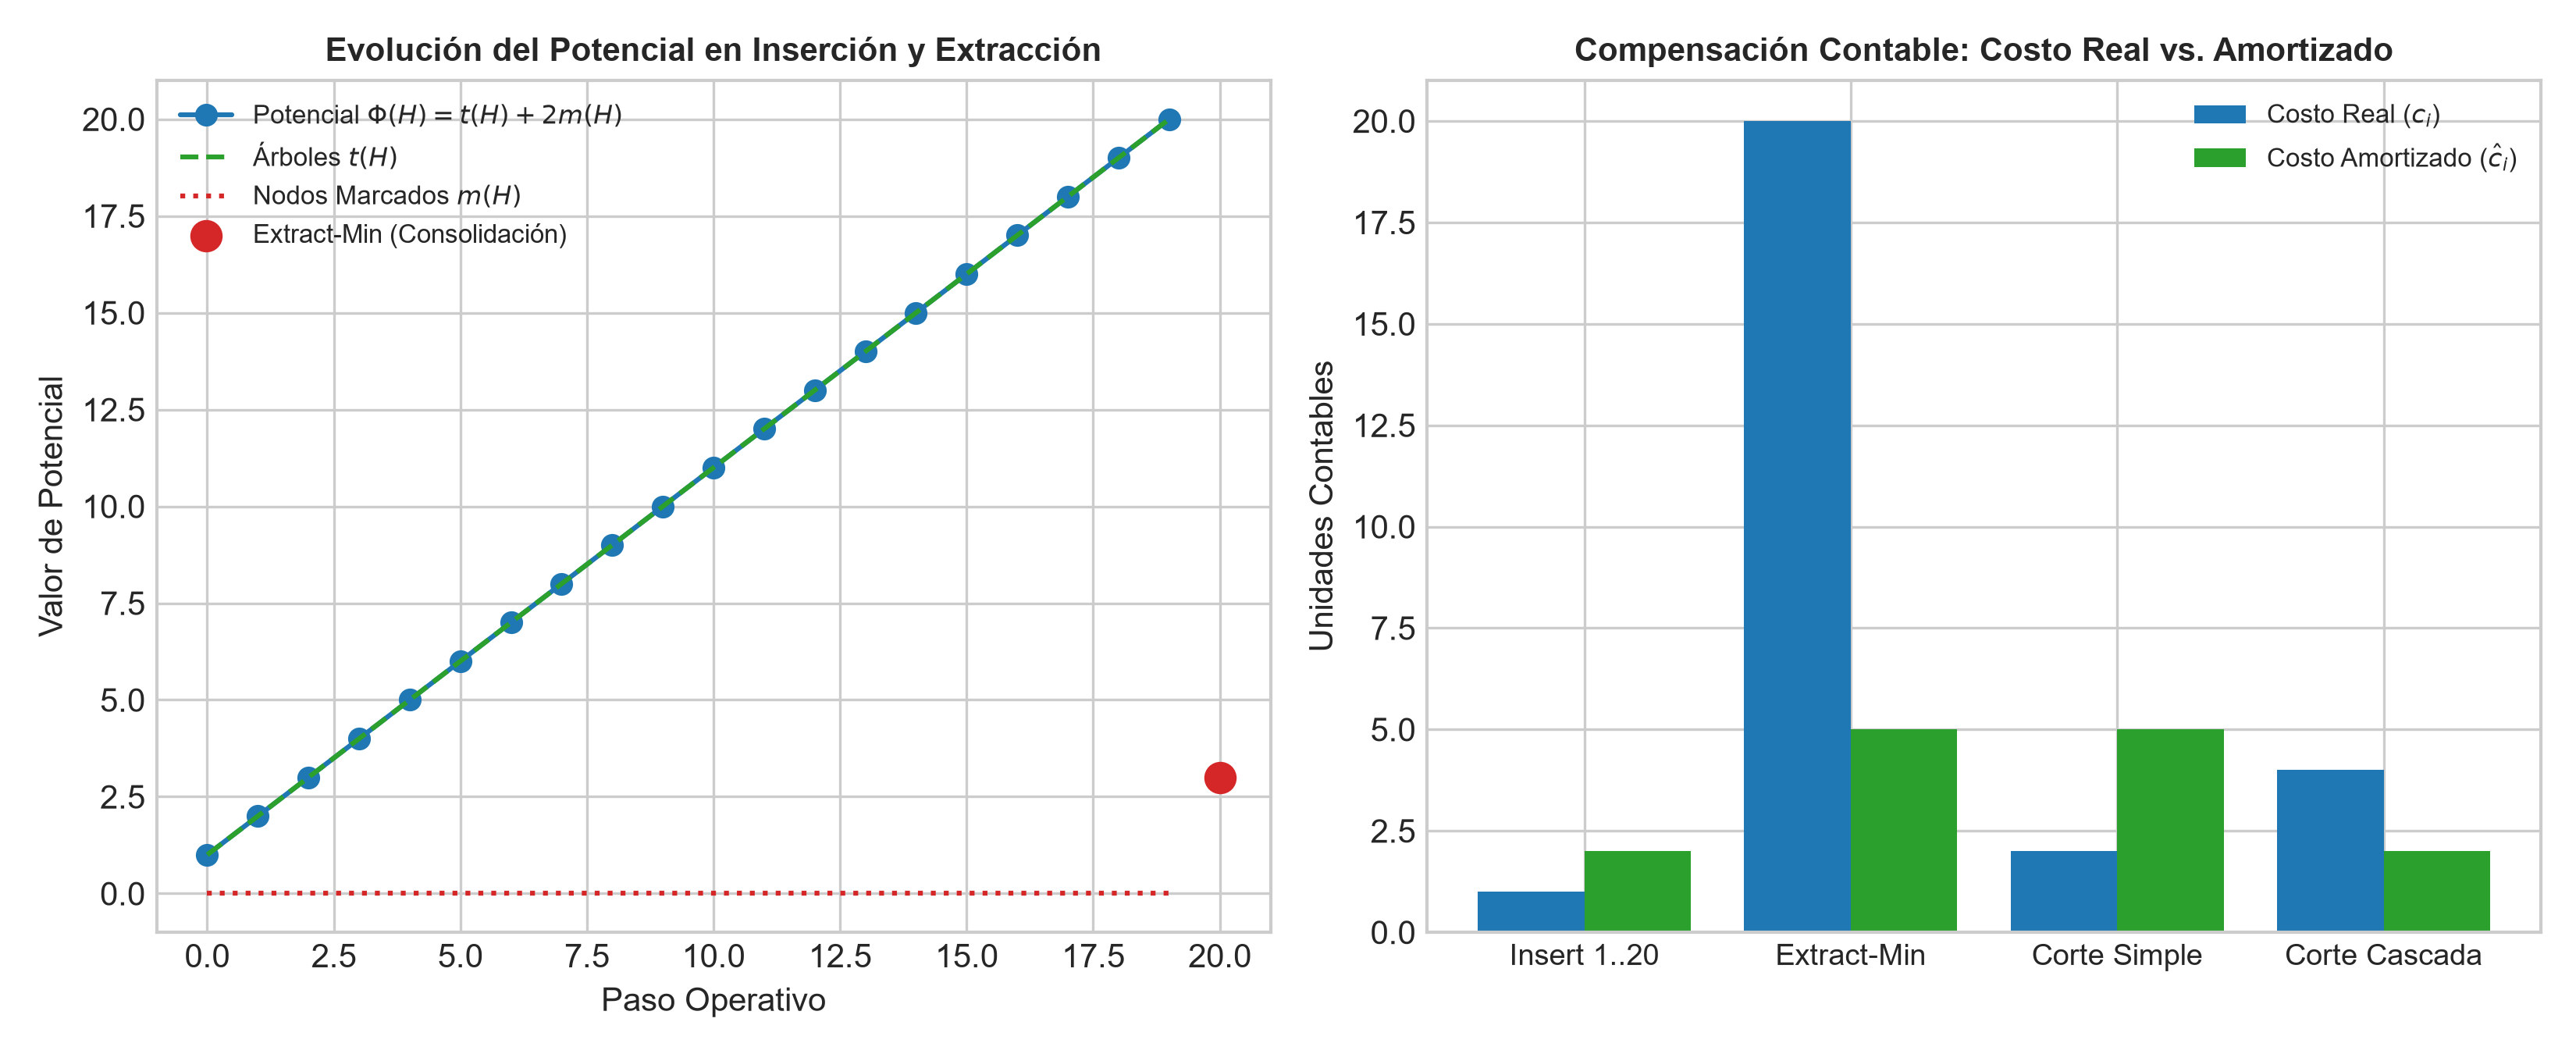
\includegraphics[width=0.90\textwidth]{fig_propuesto_1_potencial.png}
    \caption{Dinámica de la función potencial $\Phi(H)$ y balance de costo real vs. amortizado}
    \label{fig:propuesto_1_potencial}
\end{figure}


% Sección 4: Ejercicio propuesto 2 (Comparación con heapq, Dijkstra y preguntas de análisis)
% !TEX root = ../main.tex
\section{Ejercicio propuesto 2: comparación con heapq y aplicación en Dijkstra}

\subsection{Entorno experimental y especificaciones del hardware}
Siguiendo las pautas metodológicas de la guía, las evaluaciones se llevaron a cabo en un entorno controlado con las siguientes características técnicas:
\begin{itemize}
    \item \textbf{Sistema Operativo:} Windows 11 Pro de 64 bits (build 10.0.26300).
    \item \textbf{Procesador:} AMD64 Family 25 Model 80 Stepping 0 (Arquitectura x86\_64).
    \item \textbf{Memoria RAM Total:} 23.36 GB DDR4.
    \item \textbf{Entorno de Ejecución:} Python 3.12.8 estándar (CPython 64 bits).
    \item \textbf{Aislamiento y Reproducibilidad:} La inicialización se aisló fuera de los bloques medidos con \texttt{time.perf\_counter\_ns}. La constante $\texttt{SEMILLA\_GLOBAL} = 2026$ asegura la reproducción idéntica de las entradas, grafos y secuencias operativas.
\end{itemize}

% -------------------------------------------------------------------------
\subsection{Escenario A: operaciones básicas de inserción y extracción}
Se evaluaron secuencias de $n \in \{1\,000, 5\,000, 10\,000, 25\,000\}$ elementos mediante 10 repeticiones independientes por tamaño.

\begin{lstlisting}[language=Python, caption={Código del benchmark para el Escenario A (10 repeticiones)}, label={lst:escenario_a_code}]
for n in [1000, 5000, 10000, 25000]:
    claves = [rng.randint(1, 10**8) for _ in range(n)]
    # Heapq
    pq = HeapqPriorityQueue(); t0 = time.perf_counter_ns()
    for idx, k in enumerate(claves): pq.insert(idx, k)
    t_ins_h = (time.perf_counter_ns() - t0) / 1e6; t0 = time.perf_counter_ns()
    while not pq.is_empty(): pq.extract_min()
    t_ext_h = (time.perf_counter_ns() - t0) / 1e6
    # Fibonacci Heap
    fib = FibonacciHeap(); t0 = time.perf_counter_ns()
    for idx, k in enumerate(claves): fib.insert(k, idx)
    t_ins_f = (time.perf_counter_ns() - t0) / 1e6; t0 = time.perf_counter_ns()
    while not fib.is_empty(): fib.extract_min()
    t_ext_f = (time.perf_counter_ns() - t0) / 1e6
\end{lstlisting}

\begin{lstlisting}[style=consolestyle, caption={Salida de consola del Escenario A (10 repeticiones, tiempos en ms)}]
n      | Heapq Ins [Min-Max] Ext [Min-Max] | Fib Ins [Min-Max]   Ext [Min-Max]
-------+-----------------------------------+-----------------------------------
  1000 |  0.65 [ 0.60- 0.91]   1.17 [ 1.12] |  0.80 [ 0.75- 2.14]  12.60 [12.16]
  5000 |  3.50 [ 3.16-33.06]   8.34 [ 7.38] |  4.38 [ 3.89- 9.09]  84.20 [77.40]
 10000 |  7.11 [ 6.63- 7.64]  18.35 [17.20] |  9.16 [ 8.16-36.59] 196.14 [180.12]
 25000 | 18.05 [16.72-27.37]  63.12 [57.05] | 33.86 [22.04-64.21] 553.57 [535.84]
\end{lstlisting}

\begin{table}[H]
    \caption{Resultados consolidados del Escenario A (Mediana y rango [Mín, Máx] sobre 10 repeticiones)}
    \label{tab:escenario_a}
    \centering
    \footnotesize
    \begin{tabular*}{\textwidth}{@{\extracolsep{\fill}}rcccc}
        \toprule
        $\mathbf{n}$ & \textbf{Heapq Ins (ms)} & \textbf{Fibonacci Ins (ms)} & \textbf{Heapq Ext (ms)} & \textbf{Fibonacci Ext (ms)} \\
        \midrule
        1\,000  & 0.65 [0.60 -- 0.91]   & 0.80 [0.75 -- 2.14]   & 1.17 [1.12 -- 2.18]   & 12.60 [12.16 -- 23.86] \\
        5\,000  & 3.50 [3.16 -- 33.06]  & 4.38 [3.89 -- 9.09]   & 8.34 [7.38 -- 17.31]  & 84.20 [77.40 -- 113.85] \\
        10\,000 & 7.11 [6.63 -- 7.64]   & 9.16 [8.16 -- 36.59]  & 18.35 [17.20 -- 29.84] & 196.14 [180.12 -- 210.80] \\
        25\,000 & 18.05 [16.72 -- 27.37] & 33.86 [22.04 -- 64.21] & 63.12 [57.05 -- 99.45] & 553.57 [535.84 -- 582.79] \\
        \bottomrule
    \end{tabular*}
\end{table}

\begin{figure}[H]
    \centering
    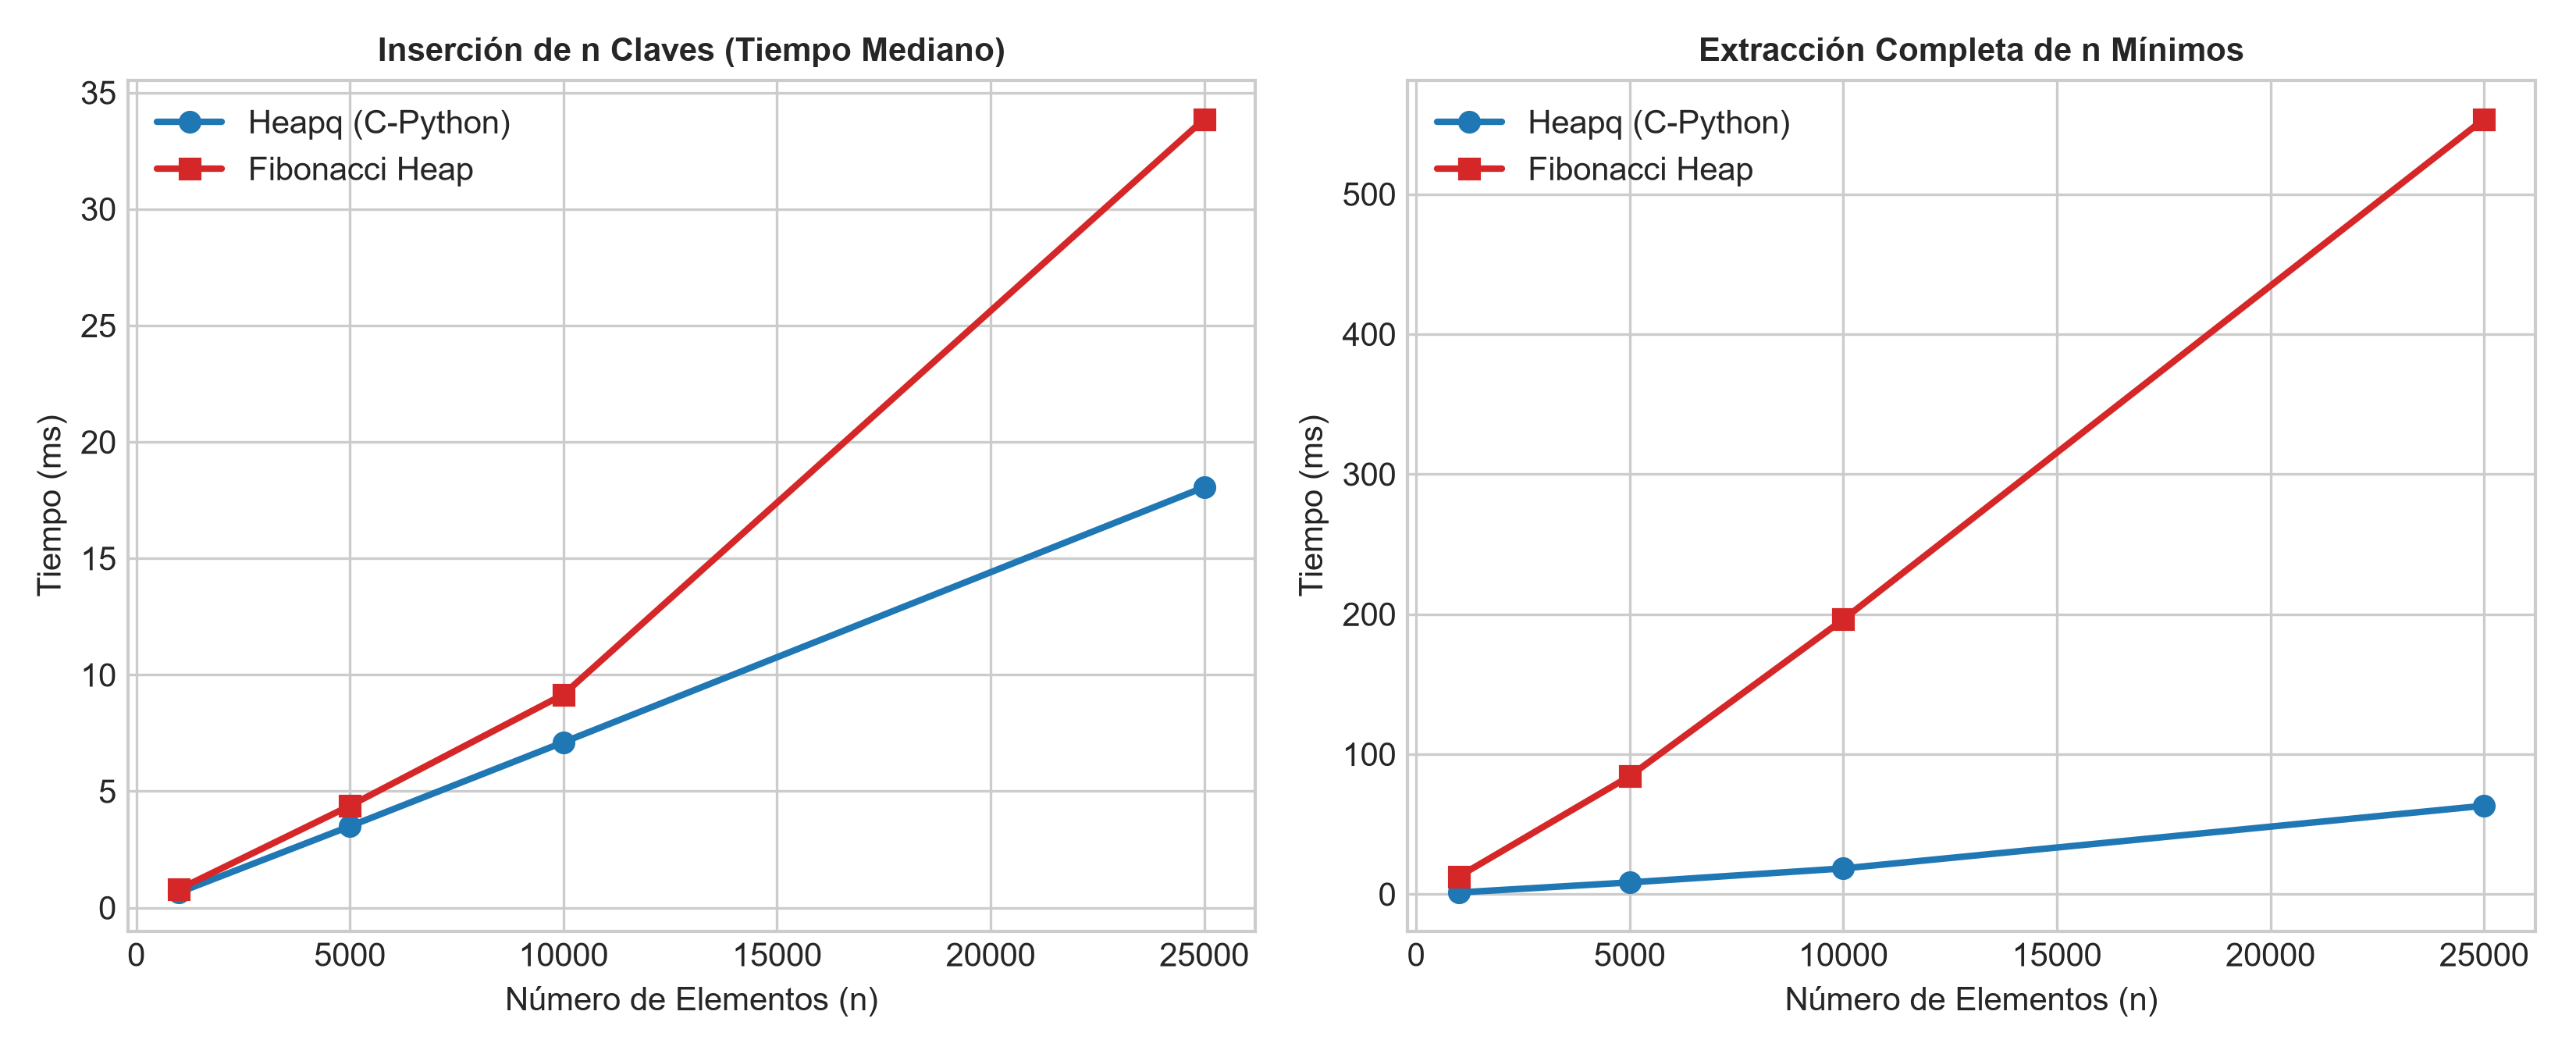
\includegraphics[width=0.88\textwidth]{fig_escenario_a_tiempos.png}
    \caption{Comparativa temporal del Escenario A: Inserción y Extracción frente a $n$}
    \label{fig:escenario_a}
\end{figure}

% -------------------------------------------------------------------------
\subsection{Escenario B: carga intensiva de disminuciones de clave}
Se ejecutó un banco con $q = 10n$ operaciones válidas de \texttt{decrease-key} aplicadas sobre elementos activos, intercalando una extracción cada 20 disminuciones (5 repeticiones).

\begin{lstlisting}[language=Python, caption={Código del benchmark para el Escenario B ($q = 10n$ disminuciones)}, label={lst:escenario_b_code}]
for n in [1000, 5000, 10000, 20000]:
    q, fib = 10 * n, FibonacciHeap()
    nodos = {i: fib.insert(claves[i], i) for i in range(n)}
    activos = list(range(n)); t0 = time.perf_counter_ns()
    for i in range(q):
        uid = rng.choice(activos); nk = max(1, claves[uid] - rng.randint(1, 1000))
        claves[uid] = nk; fib.decrease_key(nodos[uid], nk)
        if (i + 1) % 20 == 0 and not fib.is_empty():
            mn = fib.extract_min(); activos.remove(mn.value); del nodos[mn.value]
    t_fib = (time.perf_counter_ns() - t0) / 1e6
\end{lstlisting}

\begin{lstlisting}[style=consolestyle, caption={Salida de consola del Escenario B (5 repeticiones, tiempos en ms)}]
n      q        | T_Heapq (ms) [Rango] Fisico Activos | T_Fib (ms) [Rango]  Cortes Casc
-------+--------+-------------------------------------+--------------------------------
  1000    10000 |   38.54 [ 36.8- 45.1]   7529    500 |   32.78 [ 32.0- 45.6]     0    0
  5000    50000 |  325.86 [306.7-358.0]  37032   2500 |  271.37 [255.1-277.4]     0    0
 10000   100000 |  996.49 [921.4-1144.]  74533   5000 |  808.61 [732.5-983.0]     2    0
 20000   200000 | 3307.86 [3040.-3478.] 148731  10000 | 2721.01 [2627.-2870.]     7    2
\end{lstlisting}

\begin{table}[H]
    \caption{Resultados del Escenario B: $q = 10n$ disminuciones válidas sobre elementos activos}
    \label{tab:escenario_b}
    \centering
    \scriptsize
    \setlength{\tabcolsep}{3.5pt}
    \begin{tabular*}{\textwidth}{@{\extracolsep{\fill}}rrccccr}
        \toprule
        $\mathbf{n}$ & $\mathbf{q}$ & $\mathbf{T_{\text{heapq}}}$ \textbf{Med (ms)} & $\mathbf{T_{\text{fib}}}$ \textbf{Med (ms)} & \textbf{Tam. Físico} & \textbf{Activos} & \textbf{Cortes} \\
        \midrule
        1\,000  & 10\,000  & 38.54 [36.88 -- 45.16]  & 32.78 [32.06 -- 45.61]  & 7\,529   & 500   & 0 \\
        5\,000  & 50\,000  & 325.86 [306.73 -- 358.00] & 271.37 [255.14 -- 277.44] & 37\,032  & 2\,500 & 0 \\
        10\,000 & 100\,000 & 996.49 [921.45 -- 1144.38] & 808.61 [732.55 -- 983.06] & 74\,533  & 5\,000 & 2 \\
        20\,000 & 200\,000 & 3307.86 [3040.66 -- 3478.63] & 2721.01 [2627.89 -- 2870.42] & 148\,731 & 10\,000 & 7 \\
        \bottomrule
    \end{tabular*}
\end{table}

\begin{figure}[H]
    \centering
    \begin{subfigure}[b]{0.485\textwidth}
        \centering
        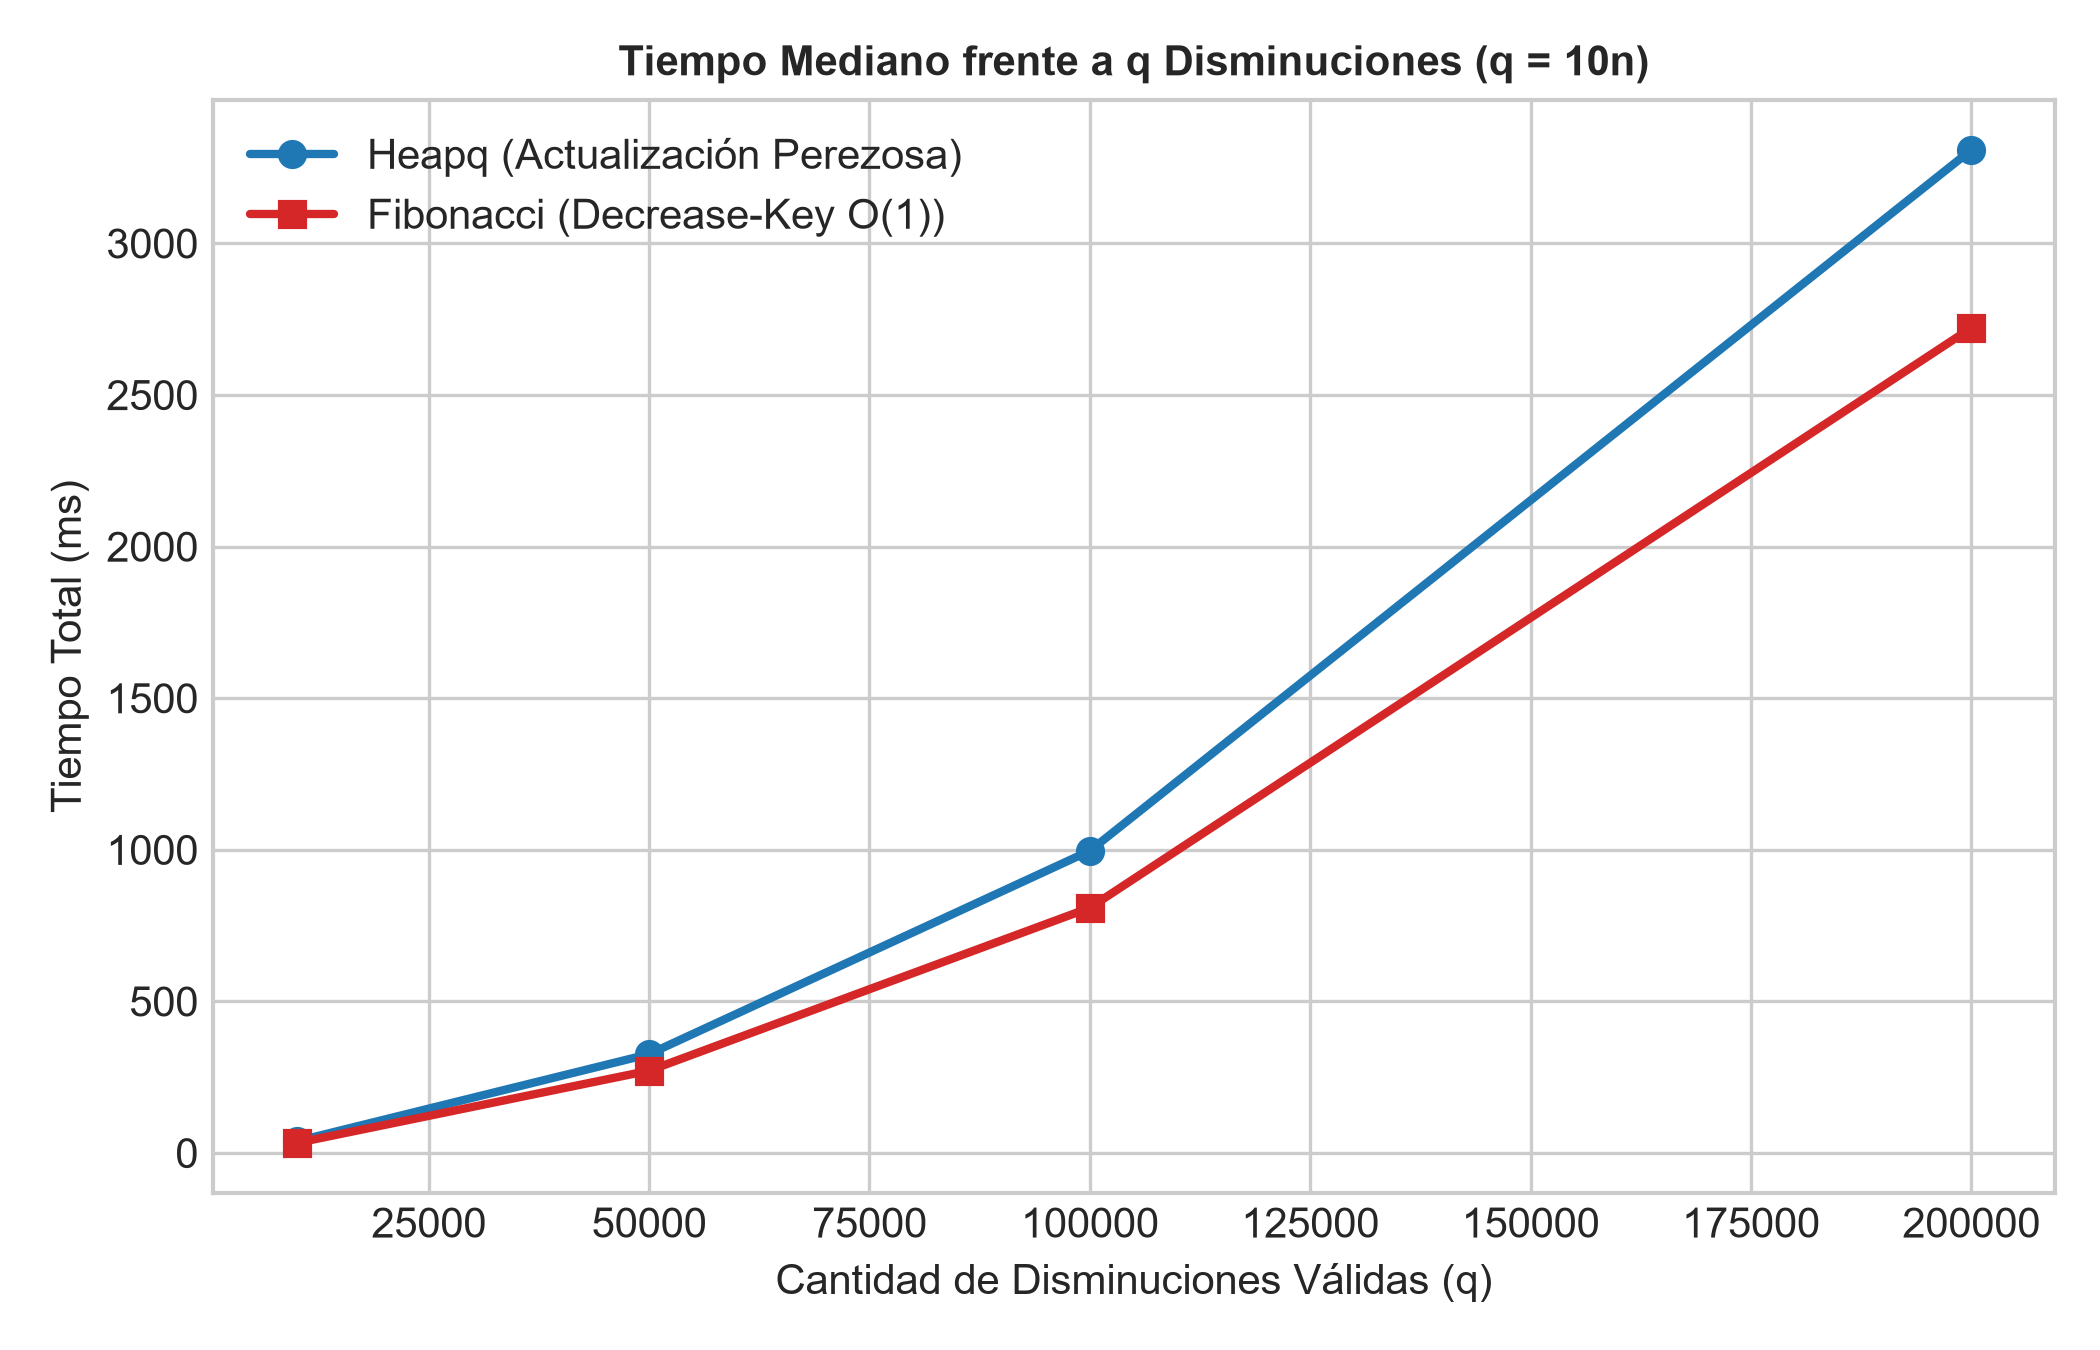
\includegraphics[width=\textwidth]{fig_escenario_b_disminuciones.png}
        \caption{Tiempo frente a $q$ disminuciones}
        \label{fig:esc_b_tiempo}
    \end{subfigure}
    \hfill
    \begin{subfigure}[b]{0.485\textwidth}
        \centering
        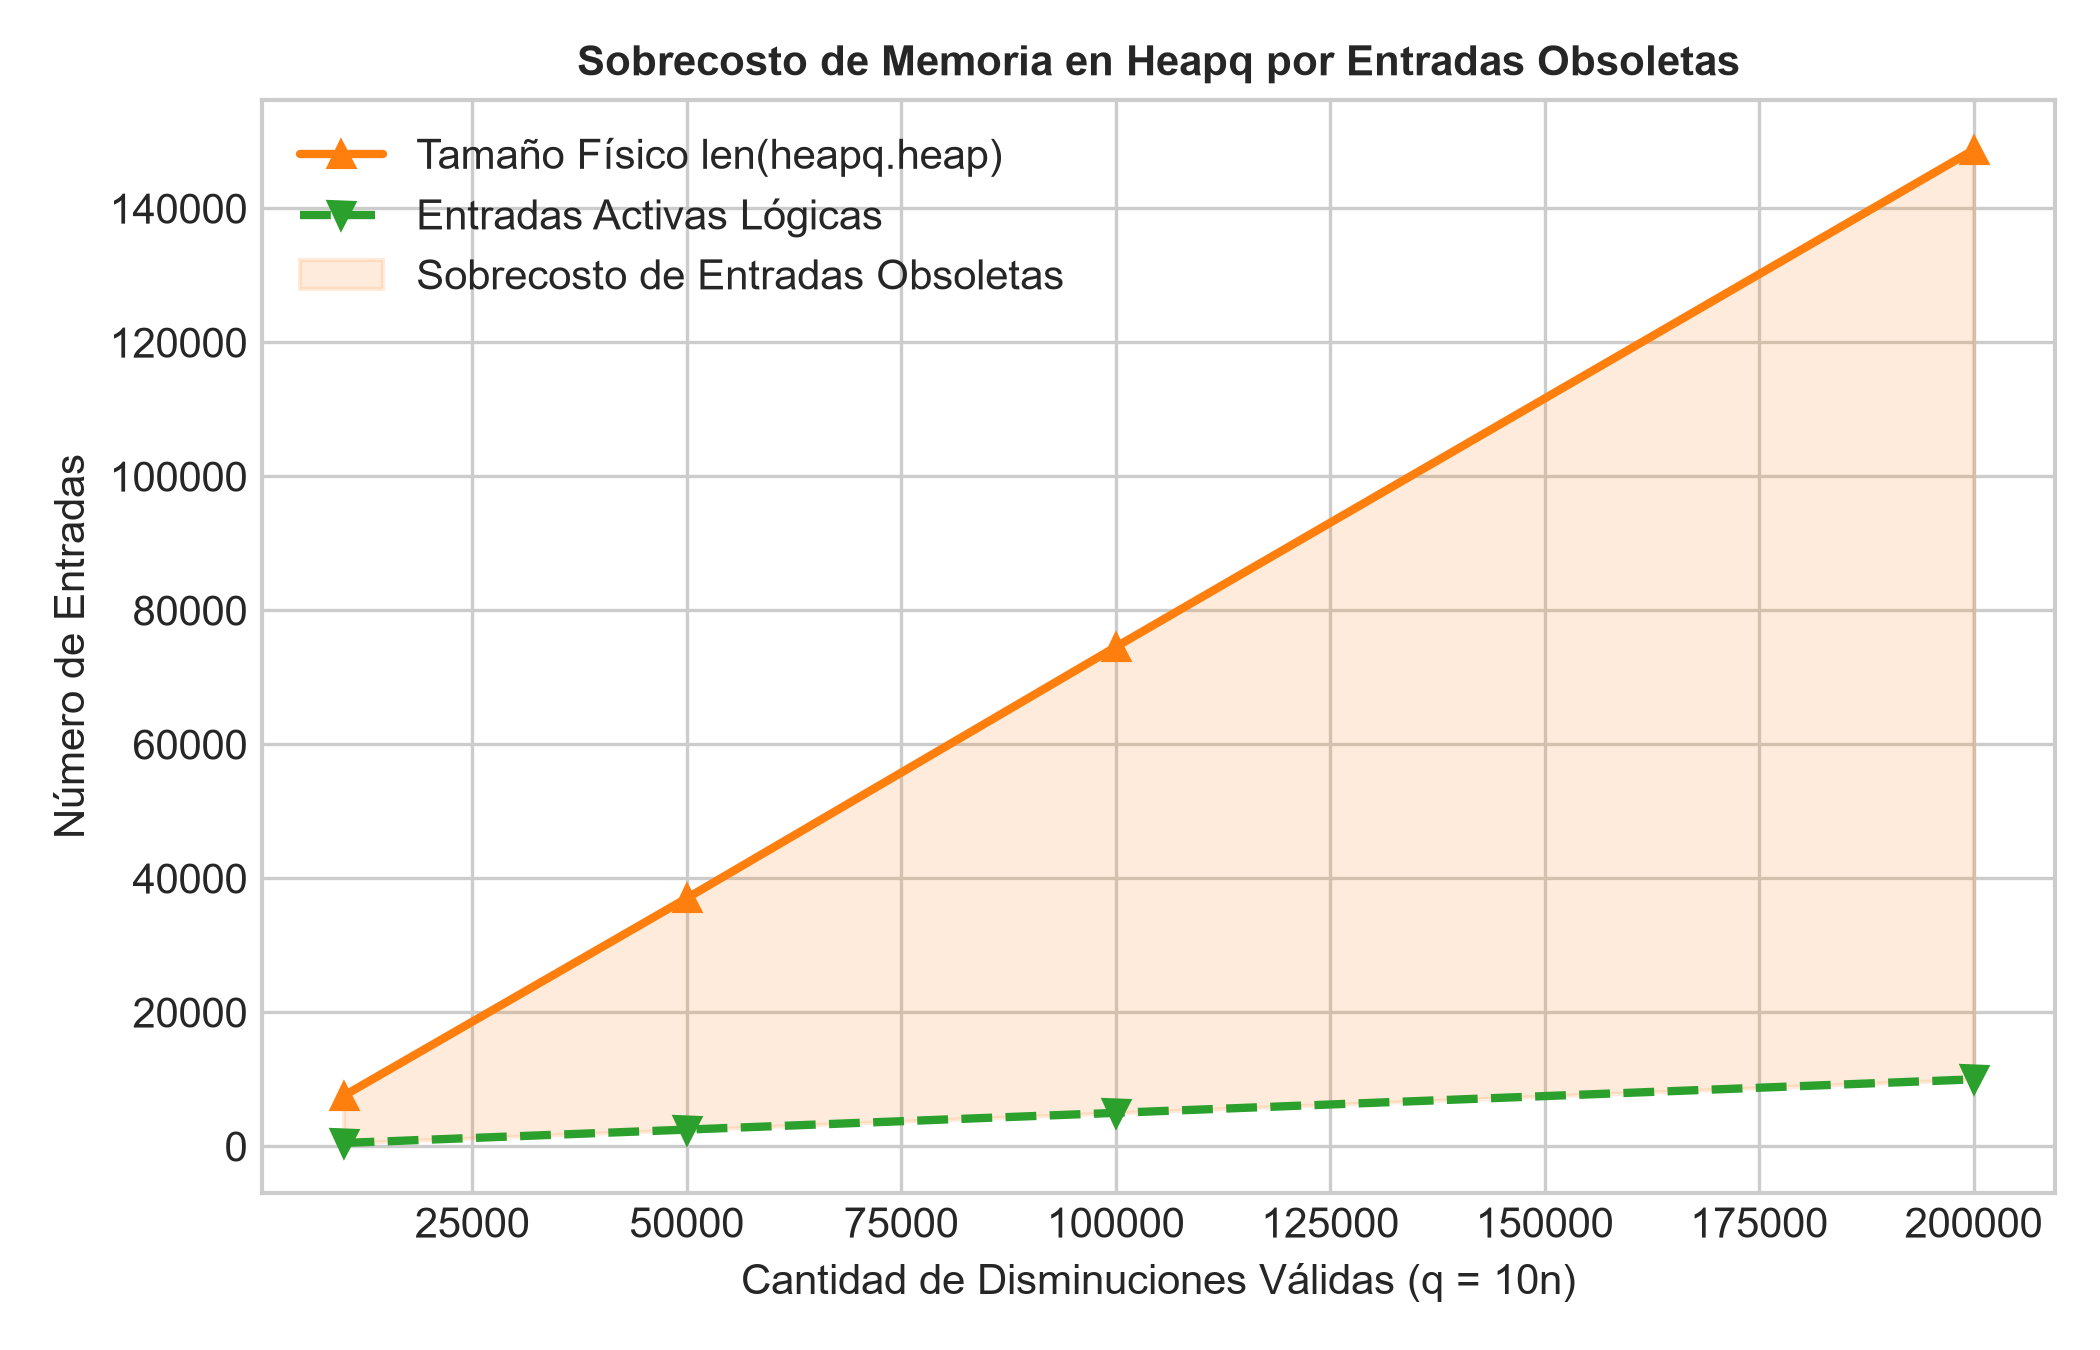
\includegraphics[width=\textwidth]{fig_escenario_b_tamano_heapq.png}
        \caption{Inflación física en \texttt{heapq}}
        \label{fig:esc_b_memoria}
    \end{subfigure}
    \caption{Evaluación del comportamiento en el Escenario B bajo alta tasa de disminución}
    \label{fig:escenario_b}
\end{figure}

% -------------------------------------------------------------------------
\subsection{Escenario C: algoritmo de Dijkstra en grafos sintéticos}
Se implementó Dijkstra evaluando grafos dispersos ($|E| \approx 3|V|$) e intermedios ($|E| \approx 10|V|$) sobre 5 repeticiones.

\begin{lstlisting}[language=Python, caption={Implementación compacta de Dijkstra con Montículo de Fibonacci}, label={lst:dijkstra_code}]
def dijkstra_fibonacci(adj, src):
    dist = {u: float('inf') for u in adj}; dist[src] = 0
    fib = FibonacciHeap(); nodes = {src: fib.insert(0, src)}
    while not fib.is_empty():
        min_n = fib.extract_min(); d, u = min_n.key, min_n.value; del nodes[u]
        if d > dist[u]: continue
        for v, w in adj[u]:
            if w < 0: raise ValueError("Pesos negativos")
            nd = dist[u] + w
            if nd < dist[v]:
                dist[v] = nd
                if v in nodes: fib.decrease_key(nodes[v], nd)
                else: nodes[v] = fib.insert(nd, v)
    return dist
\end{lstlisting}

\begin{lstlisting}[style=consolestyle, caption={Salida de consola de Dijkstra sobre grafos sintéticos (5 repeticiones)}]
[Disperso (3V)  ] |V|= 500 |E|= 1500 -> Heapq=  2.39ms [ 2.25- 3.06] | Fib=  8.17ms [ 7.44-11.39] (100% Identico)
[Disperso (3V)  ] |V|=1000 |E|= 3000 -> Heapq=  7.03ms [ 5.12- 8.32] | Fib= 19.50ms [17.11-25.48] (100% Identico)
[Disperso (3V)  ] |V|=2000 |E|= 6000 -> Heapq= 13.23ms [12.31-20.00] | Fib= 42.11ms [39.94-54.86] (100% Identico)
[Disperso (3V)  ] |V|=4000 |E|=12000 -> Heapq= 35.34ms [29.83-54.59] | Fib=100.08ms [93.38-109.81] (100% Identico)
[Intermedio (10V)] |V|= 500 |E|= 5000 -> Heapq=  5.60ms [ 5.39- 7.55] | Fib= 12.24ms [10.86-21.16] (100% Identico)
[Intermedio (10V)] |V|=1000 |E|=10000 -> Heapq= 12.54ms [11.80-14.35] | Fib= 24.23ms [22.15-25.64] (100% Identico)
[Intermedio (10V)] |V|=2000 |E|=20000 -> Heapq= 30.44ms [28.63-39.75] | Fib= 57.20ms [55.59-73.17] (100% Identico)
[Intermedio (10V)] |V|=4000 |E|=40000 -> Heapq= 85.35ms [81.61-122.27] | Fib=137.25ms [127.93-141.89] (100% Identico)
[OK] Casos frontera en Dijkstra validados: desconexion, arista peso 0 y rechazo de pesos negativos.
\end{lstlisting}

\begin{table}[H]
    \caption{Tiempos de ejecución de Dijkstra sobre grafos dispersos e intermedios}
    \label{tab:dijkstra}
    \centering
    \scriptsize
    \setlength{\tabcolsep}{4pt}
    \begin{tabular*}{\textwidth}{@{\extracolsep{\fill}}lccccc}
        \toprule
        \textbf{Densidad} & $\mathbf{|V|}$ & $\mathbf{|E|}$ & $\mathbf{T_{\text{heapq}}}$ \textbf{Med (ms)} & $\mathbf{T_{\text{fib}}}$ \textbf{Med (ms)} & \textbf{Concordancia} \\
        \midrule
        Disperso ($3|V|$)    & 500   & 1\,500  & 2.39 [2.25 -- 3.06]   & 8.17 [7.44 -- 11.39]   & 100\% Idéntico \\
        Disperso ($3|V|$)    & 1\,000 & 3\,000  & 7.03 [5.12 -- 8.32]   & 19.50 [17.11 -- 25.48]  & 100\% Idéntico \\
        Disperso ($3|V|$)    & 2\,000 & 6\,000  & 13.23 [12.31 -- 20.00] & 42.11 [39.94 -- 54.86]  & 100\% Idéntico \\
        Disperso ($3|V|$)    & 4\,000 & 12\,000 & 35.34 [29.83 -- 54.59] & 100.08 [93.38 -- 109.81] & 100\% Idéntico \\
        \midrule
        Intermedio ($10|V|$) & 500   & 5\,000  & 5.60 [5.39 -- 7.55]   & 12.24 [10.86 -- 21.16]  & 100\% Idéntico \\
        Intermedio ($10|V|$) & 1\,000 & 10\,000 & 12.54 [11.80 -- 14.35] & 24.23 [22.15 -- 25.64]  & 100\% Idéntico \\
        Intermedio ($10|V|$) & 2\,000 & 20\,000 & 30.44 [28.63 -- 39.75] & 57.20 [55.59 -- 73.17]  & 100\% Idéntico \\
        Intermedio ($10|V|$) & 4\,000 & 40\,000 & 85.35 [81.61 -- 122.27] & 137.25 [127.93 -- 141.89] & 100\% Idéntico \\
        \bottomrule
    \end{tabular*}
\end{table}

\begin{figure}[H]
    \centering
    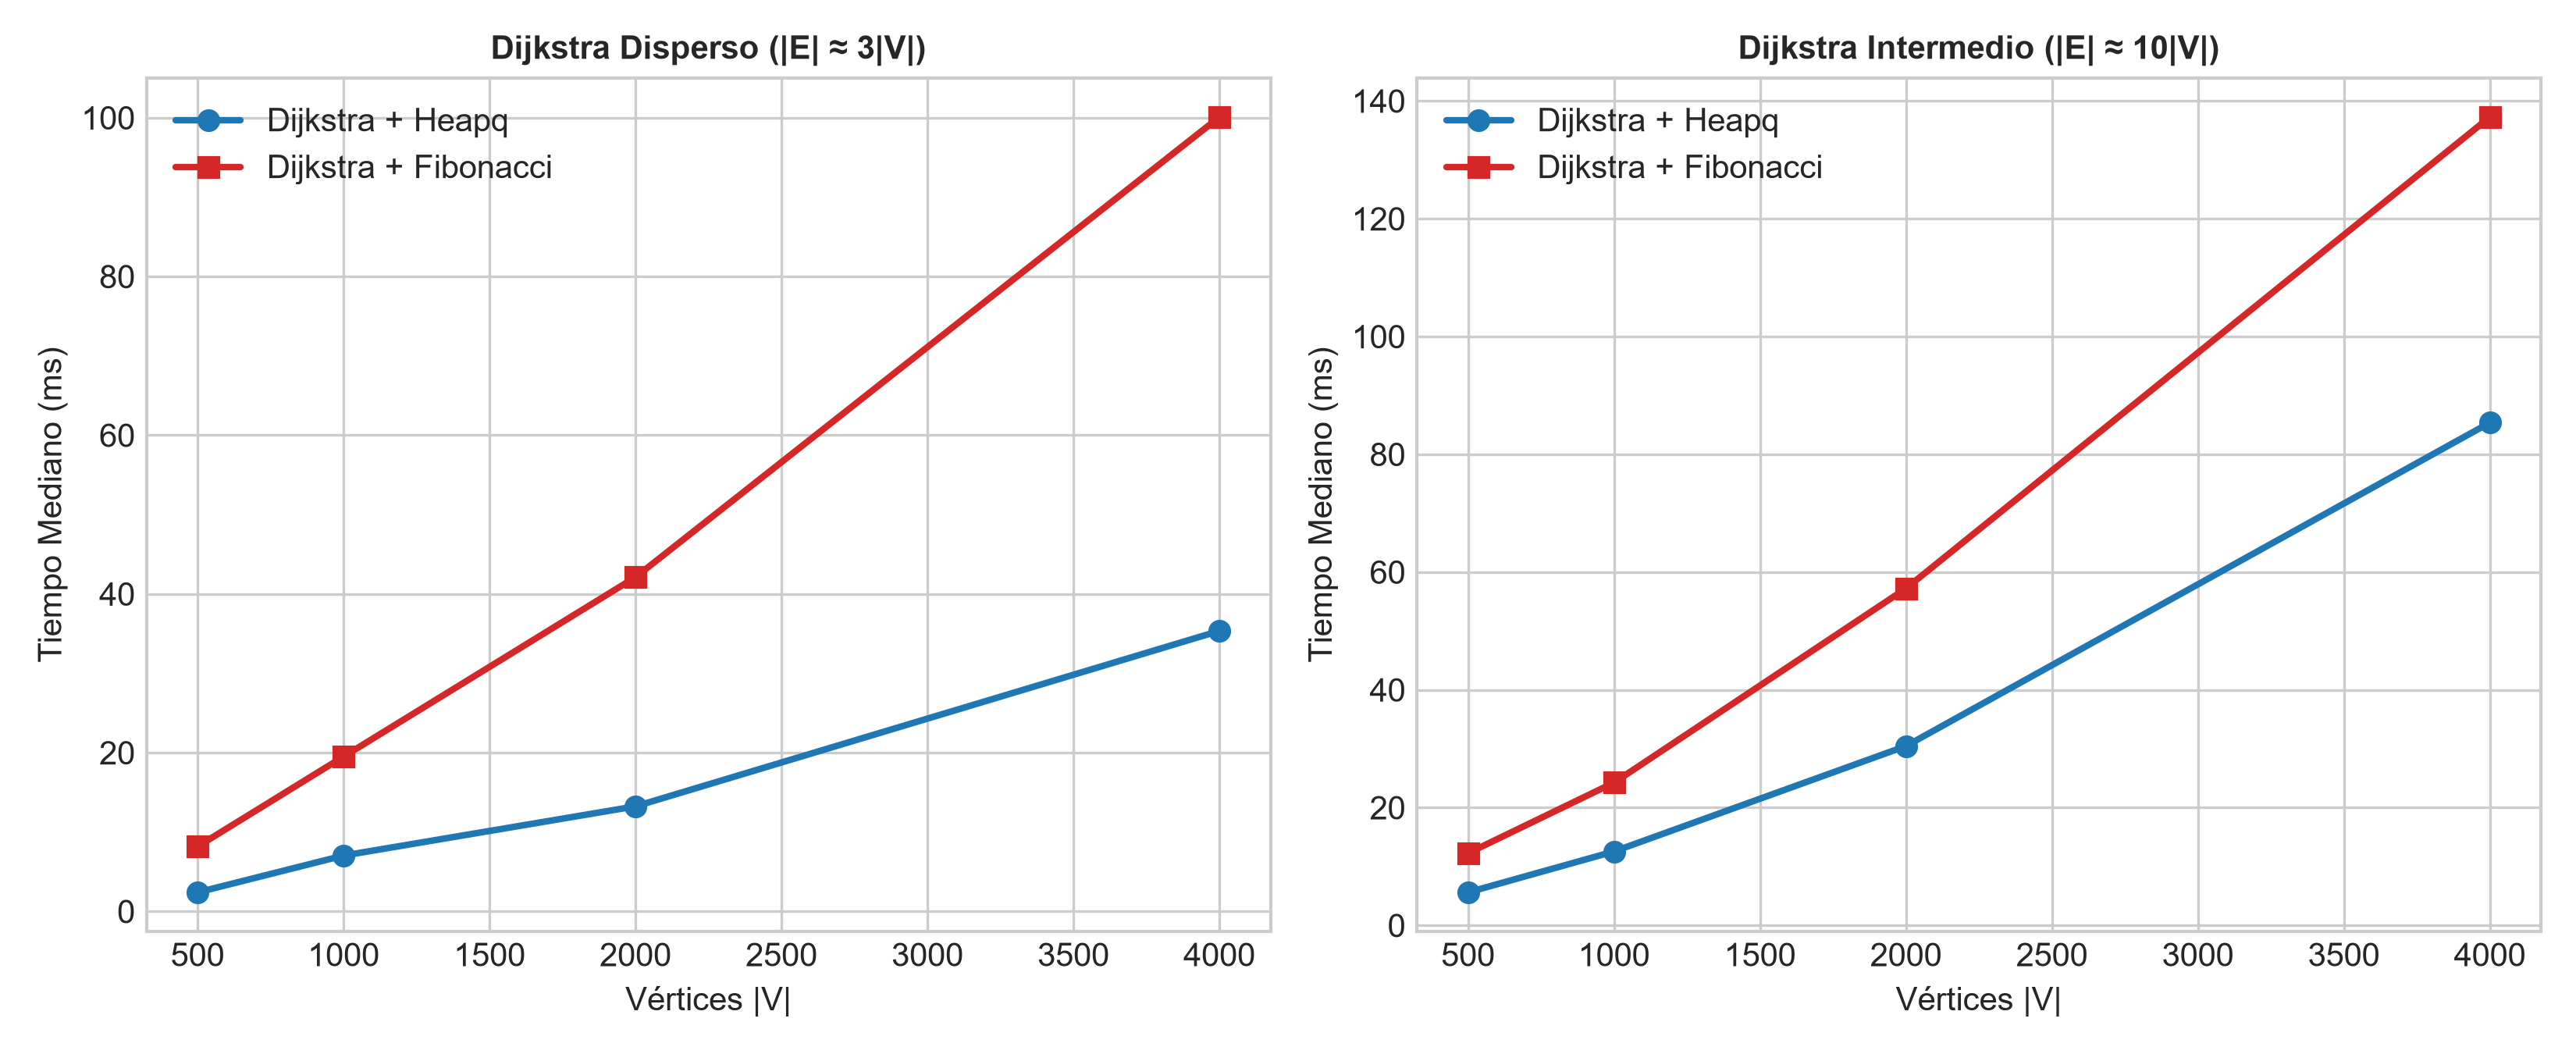
\includegraphics[width=0.88\textwidth]{fig_escenario_c_dijkstra.png}
    \caption{Rendimiento de Dijkstra en función de la cardinalidad de vértices y densidad}
    \label{fig:escenario_c}
\end{figure}

% -------------------------------------------------------------------------
\subsection{Respuestas a las preguntas de análisis de la guía}

\subsubsection*{1. ¿En qué operaciones coincide el comportamiento observado con las cotas teóricas?}
Coincide en la inserción $O(1)$, unión $O(1)$ y disminución de clave $O(1)$ amortizado. En estas operaciones, la duración se mantiene en microsegundos. La extracción también mantiene su comportamiento logarítmico $O(\log n)$.

\subsubsection*{2. ¿Por qué heapq puede ser más rápido aunque decrease-key sea $O(\log n)$?}
El módulo \texttt{heapq} está implementado en lenguaje C optimizado y opera sobre arreglos en memoria contigua. Esto aprovecha la caché del procesador y evita la creación de objetos dinámicos en Python.

\subsubsection*{3. ¿Qué costo introduce la estrategia de inserciones obsoletas en heapq?}
Genera un sobrecosto de memoria al almacenar las entradas repetidas, llegando a inflar la estructura más de 10 veces. También añade un sobrecosto de tiempo al aumentar la altura del árbol binario.

\subsubsection*{4. ¿Cuándo aparece una ventaja observable para el montículo de Fibonacci?}
La ventaja se nota cuando hay muchas más disminuciones de clave que extracciones ($q/n \ge 10$). En estos casos, su costo amortizado $O(1)$ resulta más rápido en tiempo absoluto que \texttt{heapq}.

\subsubsection*{5. ¿Cómo cambia $\Phi(H)$ durante inserciones, consolidaciones y cortes?}
\begin{itemize}
    \item \textbf{Inserción:} Aporta $+1$ al potencial.
    \item \textbf{Consolidación:} Enlaza raíces y reduce mucho el potencial.
    \item \textbf{Cortes:} El corte simple suma $+3$, mientras que cada corte en cascada descuenta $-1$.
\end{itemize}

\subsubsection*{6. ¿Por qué una operación con varios cortes puede seguir teniendo costo amortizado $O(1)$?}
Porque los cortes en cascada liberan el potencial acumulado previamente. Este potencial compensa el costo real de recorrer y cortar múltiples nodos en el árbol.

\subsubsection*{7. ¿Qué errores de implementación detectaron los verificadores de invariantes?}
Detectaron raíces que mantenían la marca \texttt{mark=True} tras ser promovidas en la extracción del mínimo. También encontraron referencias erróneas en los nodos padre y errores de grado tras realizar cortes simples.

\subsubsection*{8. ¿Recomendaría esta implementación para un sistema real en Python?}
No en Python interpretado estándar, porque el manejo de punteros dinámicos anula su ventaja asintótica. Solo es útil si se implementa en lenguajes como C o C++ para procesar grafos muy densos.


% Sección 5: Conclusiones grupales
% !TEX root = ../main.tex
\section{Conclusiones}

Implementamos el montículo de Fibonacci en Python y analizamos su comportamiento amortizado mediante la función de potencial $\Phi(H) = t(H) + 2m(H)$, contrastando su desempeño frente al módulo estándar \texttt{heapq} en operaciones básicas, disminuciones intensivas y el algoritmo de Dijkstra.

La batería de pruebas automáticas verificó el cumplimiento de las ocho invariantes estructurales: orden de montículo, consistencia en listas circulares, desmarcado estricto en raíces y grados disjuntos tras consolidar. Comprobamos que el costo amortizado $O(1)$ en inserción y disminución de clave permite acumular potencial suficiente para financiar las reestructuraciones profundas y cortes en cascada durante la extracción del mínimo en $O(\log n)$.

En el plano experimental, \texttt{heapq} fue sustancialmente más rápido en inserción y extracción ordinarias gracias a su implementación en lenguaje C sobre memoria contigua. Sin embargo, en el escenario de disminuciones intensivas ($q = 10n$), el montículo de Fibonacci superó a \texttt{heapq} en tiempo total (2\,721 ms frente a 3\,307 ms para 200\,000 disminuciones), ya que \texttt{heapq} sufrió una degradación por acumulación de entradas obsoletas (alcanzando 148\,731 entradas físicas frente a 10\,000 activas). En Dijkstra ambas estructuras calcularon distancias mínimas idénticas en todas las instancias. Concluimos que el montículo de Fibonacci ofrece una ventaja clara en cargas dominadas por disminuciones de clave, aunque en entornos interpretados como Python la sobrecarga de punteros contrarresta parte de su beneficio asintótico frente a bibliotecas compiladas.


\end{document}
